\section{Example Scenario}
\label{sec:Example}

\begin{figure*}
    \centering
    \begin{subfigure}[b]{0.45\textwidth}
			\centering
      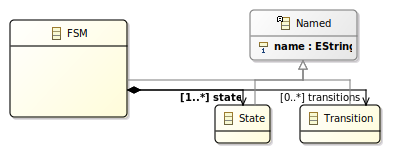
\includegraphics[width=\textwidth]{FSM0.pdf}
      \caption{Initial \metamodel.}
      \label{fig:FSM:Init}
    \end{subfigure}
    \hfill
    \begin{subfigure}[b]{0.45\textwidth}
			\centering
      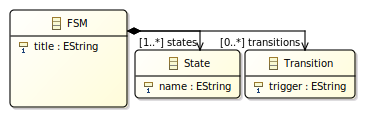
\includegraphics[width=\textwidth]{FSM1.pdf}
      \caption{First evolution: putting relevant names}
      \label{fig:FSM:Relevant}
    \end{subfigure}
    \hfill
    \begin{subfigure}[b]{0.45\textwidth}
			\centering
      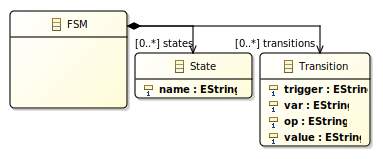
\includegraphics[width=\textwidth]{FSM2.pdf}
      \caption{Second evolution: introducing rudimentary guards.}
      \label{fig:FSM:Guard}
    \end{subfigure}
    \hfill 
		\begin{subfigure}[b]{0.45\textwidth}
			\centering
      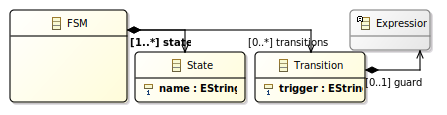
\includegraphics[width=\textwidth]{FSM3.pdf}
      \caption{Third evolution: Fully-fledged expressions for \textsf{guard}s.}
      \label{fig:FSM:Expression}
    \end{subfigure}
    \caption{Three evolution steps for the \textsf{FSM} \metamodel}
    \label{fig:FSM}
\end{figure*}


\MA{Not finished yet! It needs:
\begin{itemize}
	\item Figures for views;
	\item Eventually, explanation that all is synced with the internal model.
	\item Explanation on the impact of the changes
\end{itemize}
Note that I completely failed at finding evolution steps that are purely ``atomic'':
any \emph{meaningful} (in the sense of my explanation here) evolution step, even
for such a small example, actually uses \textbf{a list of} atomic/composite 
changes!!! This was only partially discussed in our last meeting...}

This Section describes a small, yet representative example of \metamodel
evolution steps on a popular \textsc{Dsl}, the Finite State Machine (\textsf{FSM}).
Note that we simplify the \metamodels and corresponding \viewtypes, to focus 
the discussion only on the parts relevant to co-evolution. 

A methodologist starts with a very simple version, where an \textsf{FSM} consists
of \textsf{State}s and \textsf{Transition}s: each inherits a \textsf{name} for
identifying the \textsf{State}s, and specifying which action triggers a 
\textsf{Transition}. This version allows to build two simple views. A \emph{visual}
editor allows to create and edit \textsf{FSM}s, using \textsf{Rountangle}s and
\textsf{Arrow}s, and constantly displaying the total number of \textsf{State}s
and \textsf{Transition}s. A \emph{textual} view offers a read-only representation
where \textsf{Transition}s are ``embedded'' inside \textsf{State}s. 
%
Noticing that the \textsf{name}s play different roles for each class, the methodologist
improves the \metamodel by \emph{pushing down} the \textsf{name}s, and specialising
the one in \textsf{Transition} (thus naming it \textsf{trigger}). This evolution
step does not have a consequence on the \viewtypes; however, the way views are
computed needs to evolve as well (e.g. accessing a \textsf{Transition}'s trigger
changed from \texttt{self.name} to \texttt{self.\textbf{trigger}}).
%
Now, the methodologist wants to add new behaviour to the \metamodel, and adds
a rudimentary representation of guards, by \emph{creating (new) attributes}
in \textsf{Transition}, allowing to capture simple expressions over 
\textsf{var}iables, using boolean and numeric \textsf{value}s
(e.g. \textsf{v = 10} or \textsf{k or l}). While previous models may still be valid
wrt. the evolved \metamodel (if the lack of guard is interpreted as \textsf{true}),
\viewtypes need to reflect this new information by adding new entities. 
%
Finally, the methodologist defines a fully-fledged \textsf{Expression} model,
allowing a \textsf{Transition} to possess a \textsf{guard}, after deleting the
three attributes \textsf{var}, \textsf{op} and \textsf{value} in \textsf{Transition}.
